\begin{exercice*}
    Voici un organigramme.

    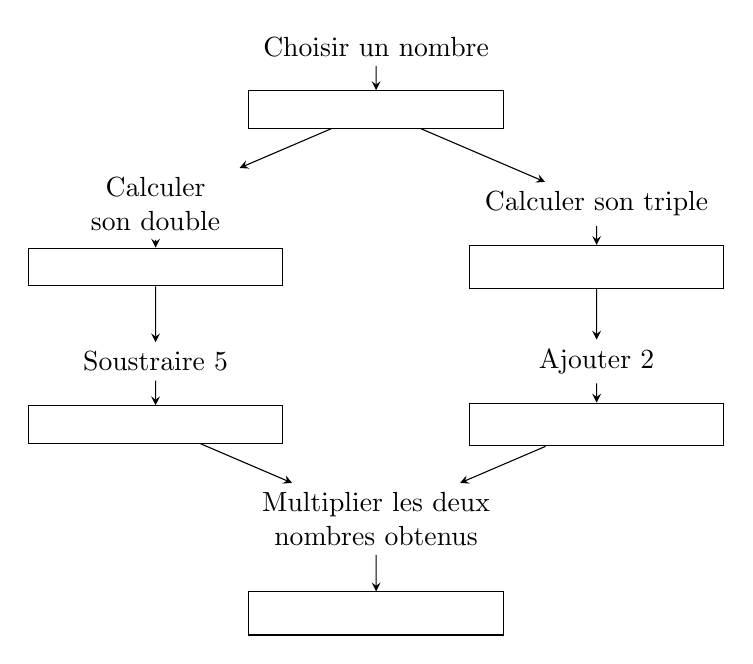
\begin{tikzpicture}[>=stealth,yscale=2,xscale=1.4]  
        % xscale et yscale permettent d'ajuster largeur et hauteur
        
        % positionner les nœuds
        \node(etape1) at (4,3)[text width=3cm,text centered] {Choisir un nombre};
        \node(etape1cadre) at (4,2.6)[rectangle,draw,text width=3cm,text centered] {\phantom{Choisir un nombre}};
        \node(etape2g) at (2,2)[text width=3cm,text centered] {Calculer son double};
        \node(etape2gcadre) at (2,1.6)[text width=3cm,rectangle,draw] {\phantom{Calculer son double}};
        \node(etape2d) at (6,2)[text width=3cm,text centered] {Calculer son triple};
        \node(etape2dcadre) at (6,1.6)[text width=3cm,rectangle,draw] {\phantom{Calculer son triple}};
        \node(etape3g) at (2,1)[text width=3cm,text centered] {Soustraire $5$};
        \node(etape3gcadre) at (2,0.6)[text width=3cm,rectangle,draw] {\phantom{Soustraire $5$}};
        \node(etape3d) at (6,1)[text width=3cm,text centered] {Ajouter $2$};
        \node(etape3dcadre) at (6,0.6)[text width=3cm,rectangle,draw] {\phantom{Ajouter $2$}};
        \node(etape4) at (4,0)[text width=3cm,text centered] {Multiplier les deux\\nombres obtenus};
        \node(etape4cadre) at (4,-0.6)[text width=3cm,rectangle,draw] {\phantom{Multiplier les deux}};
                              
        % tirer les liens
        \draw[->] (etape1) -- (etape1cadre);
        \draw[->] (etape1cadre) -- (etape2g); 
        \draw[->] (etape2g) -- (etape2gcadre);
        \draw[->] (etape1cadre) -- (etape2d); 
        \draw[->] (etape2d) -- (etape2dcadre);
        \draw[->] (etape2gcadre) -- (etape3g); 
        \draw[->] (etape3g) -- (etape3gcadre);
        \draw[->] (etape2dcadre) -- (etape3d); 
        \draw[->] (etape3d) -- (etape3dcadre);
        \draw[->] (etape3gcadre) -- (etape4);
        \draw[->] (etape3dcadre) -- (etape4);
        \draw[->] (etape4) -- (etape4cadre);
    \end{tikzpicture}
    \begin{enumerate}
        \item Montrer que le résultat final vaut $-15$ si on prend $1$ au départ.
        \item Parmi les expressions suivantes, déterminer celle que l'on obtient en partant d'un nombre quelconque $x$.\\
            $A=(x^2-5)\times(3x+2)$ \hfill $B=(2x-5)\times (3x+2)$\hfill $C=2x-5\times3x+2$
        \item Lily prétend que $D=(3x+2)^2-(x+7)(3x+2)$ donne les mêmes résultats que $B$ pour toutes les valeurs de $x$. Déterminer si son affirmation est vraie. Justifier.
    \end{enumerate}
\end{exercice*}
\begin{corrige}
    %\setcounter{partie}{0} % Pour s'assurer que le compteur de \partie est à zéro dans les corrigés
    %\phantom{rrr}    
    \begin{enumerate}
        \item Montrer que le résultat final vaut $-15$ si on prend $1$ au départ.\\
        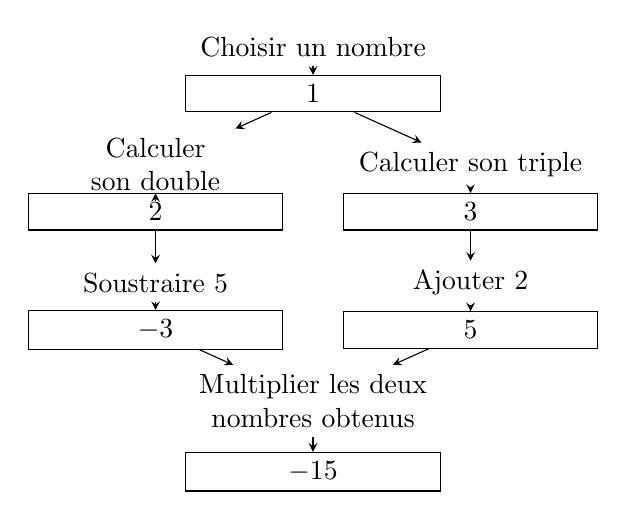
\begin{tikzpicture}[>=stealth,yscale=1.5,xscale=1]  
            % xscale et yscale permettent d'ajuster largeur et hauteur
            
            % positionner les nœuds
            \node(etape1) at (4,3)[text width=3cm,text centered] {Choisir un nombre};
            \node(etape1cadre) at (4,2.6)[rectangle,draw,text width=3cm,text centered] {{\red $1$}};
            \node(etape2g) at (2,2)[text width=3cm,text centered] {Calculer son double};
            \node(etape2gcadre) at (2,1.6)[text width=3cm,rectangle,draw,text centered] {{\red $2$}};
            \node(etape2d) at (6,2)[text width=3cm,text centered] {Calculer son triple};
            \node(etape2dcadre) at (6,1.6)[text width=3cm,rectangle,draw,text centered] {{\red $3$}};
            \node(etape3g) at (2,1)[text width=3cm,text centered] {Soustraire $5$};
            \node(etape3gcadre) at (2,0.6)[text width=3cm,rectangle,draw,text centered] {{\red $-3$}};
            \node(etape3d) at (6,1)[text width=3cm,text centered] {Ajouter $2$};
            \node(etape3dcadre) at (6,0.6)[text width=3cm,rectangle,draw,text centered] {{\red $5$}};
            \node(etape4) at (4,0)[text width=3cm,text centered] {Multiplier les deux\\nombres obtenus};
            \node(etape4cadre) at (4,-0.6)[text width=3cm,rectangle,draw,text centered] {{\red $-15$}};
                                  
            % tirer les liens
            \draw[->] (etape1) -- (etape1cadre);
            \draw[->] (etape1cadre) -- (etape2g); 
            \draw[->] (etape2g) -- (etape2gcadre);
            \draw[->] (etape1cadre) -- (etape2d); 
            \draw[->] (etape2d) -- (etape2dcadre);
            \draw[->] (etape2gcadre) -- (etape3g); 
            \draw[->] (etape3g) -- (etape3gcadre);
            \draw[->] (etape2dcadre) -- (etape3d); 
            \draw[->] (etape3d) -- (etape3dcadre);
            \draw[->] (etape3gcadre) -- (etape4);
            \draw[->] (etape3dcadre) -- (etape4);
            \draw[->] (etape4) -- (etape4cadre);
        \end{tikzpicture}
        \item Parmi les expressions suivantes, déterminer celle que l'on obtient en partant d'un nombre quelconque $x$.\\
            $A=(x^2-5)\times(3x+2)$ \hfill $B=(2x-5)\times (3x+2)$\hfill $C=2x-5\times3x+2$\\
            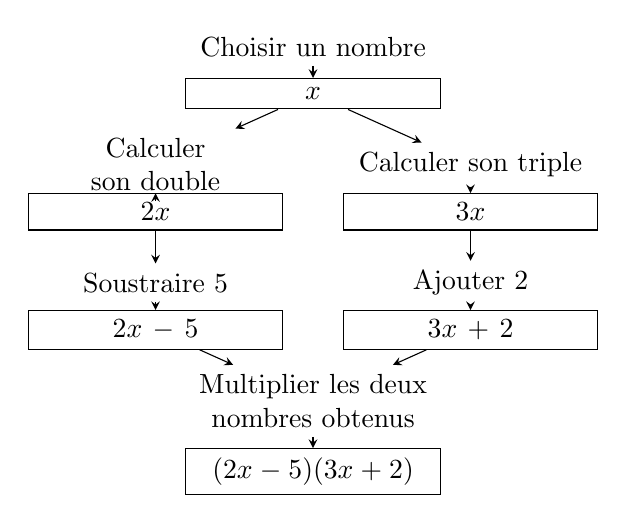
\begin{tikzpicture}[>=stealth,yscale=1.5,xscale=1]  
                % xscale et yscale permettent d'ajuster largeur et hauteur
                
                % positionner les nœuds
                \node(etape1) at (4,3)[text width=3cm,text centered] {Choisir un nombre};
                \node(etape1cadre) at (4,2.6)[rectangle,draw,text width=3cm,text centered] {{\red $x$}};
                \node(etape2g) at (2,2)[text width=3cm,text centered] {Calculer son double};
                \node(etape2gcadre) at (2,1.6)[text width=3cm,rectangle,draw,text centered] {{\red $2x$}};
                \node(etape2d) at (6,2)[text width=3cm,text centered] {Calculer son triple};
                \node(etape2dcadre) at (6,1.6)[text width=3cm,rectangle,draw,text centered] {{\red $3x$}};
                \node(etape3g) at (2,1)[text width=3cm,text centered] {Soustraire $5$};
                \node(etape3gcadre) at (2,0.6)[text width=3cm,rectangle,draw,text centered] {{\red $2x-5$}};
                \node(etape3d) at (6,1)[text width=3cm,text centered] {Ajouter $2$};
                \node(etape3dcadre) at (6,0.6)[text width=3cm,rectangle,draw,text centered] {{\red $3x+2$}};
                \node(etape4) at (4,0)[text width=3cm,text centered] {Multiplier les deux\\nombres obtenus};
                \node(etape4cadre) at (4,-0.6)[text width=3cm,rectangle,draw,text centered] {{\red $(2x-5)(3x+2)$}};
                                      
                % tirer les liens
                \draw[->] (etape1) -- (etape1cadre);
                \draw[->] (etape1cadre) -- (etape2g); 
                \draw[->] (etape2g) -- (etape2gcadre);
                \draw[->] (etape1cadre) -- (etape2d); 
                \draw[->] (etape2d) -- (etape2dcadre);
                \draw[->] (etape2gcadre) -- (etape3g); 
                \draw[->] (etape3g) -- (etape3gcadre);
                \draw[->] (etape2dcadre) -- (etape3d); 
                \draw[->] (etape3d) -- (etape3dcadre);
                \draw[->] (etape3gcadre) -- (etape4);
                \draw[->] (etape3dcadre) -- (etape4);
                \draw[->] (etape4) -- (etape4cadre);
            \end{tikzpicture}
            {\red C'est donc l'expression $B$.}
        \item Lily prétend que $D=(3x+2)^2-(x+7)(3x+2)$ donne les mêmes résultats que $B$ pour toutes les valeurs de $x$. Déterminer si son affirmation est vraie. Justifier.\\
        {\red $D=(3x+2)^2-(x+7)(3x+2)$\\$D=(3x+2)[(3x+2)-(x+7)]$\\$D=(3x+2)(3x+2-x-7)$\\$D=(3x+2)(2x-5)$\\ 
        $B=(2x-5)(3x+2)$ et $D=(3x+2)(2x-5)$ sont bien deux expressions égales.}
    \end{enumerate}
\end{corrige}

